% chapters/05b_cosmos.tex

\chapter{Video-Augmentierung mit Cosmos}
\label{chap:cosmos}
\label{sec:augmentierung}

Dieses Teilprojekt (federführend Maximilian Berger, \cref{tab:beitraege}) schafft neben dem
Rendering in Isaac~Lab eine zweite Quelle zusätzlicher Trainingsbilder: Echte Trainingsvideos
werden mit Cosmos-Transfer2.5~\cite{cosmostransfer2025} in Licht, Hintergrund und Oberflächen
variiert. Die Pipeline ist gebaut und lief im September 2026 einmal vollständig durch; ein
Trainingslauf mit ihren Daten steht noch aus. Befehle und Parameter stehen in
\doc{docs/augmentation/anleitung.md}.

\section{Ausgangspunkt und Ansatz}
\label{sec:cosmos-motivation}
\label{sec:cosmos-ansatz}

Das Teilprojekt entstand im August 2026, als der visuelle Domain-Gap als Hauptursache für das
Scheitern in der Simulation galt (Läufe 31--34). Inzwischen ist er direkt gemessen: Auf
Sim-Bildern ist der Fehler der Hand-Aktionen 13- bzw.\ 36-mal so groß wie auf echten
(\cref{sec:erg-domain-gap}). Während das Rendering (\cref{sec:erg-cotrain}) Sim-Bilder erzeugt,
nimmt Cosmos die echten Videos und ändert nur ihr Aussehen. Die Bewegung bleibt identisch,
sodass die aufgezeichneten Aktionen unverändert passen. Das ist \ac{dr}~\cite{tobin2017domain}
auf echten Daten: Die Policy soll lernen, Licht, Hintergrund und Oberflächen zu ignorieren.

\section{Modell und Pipeline}
\label{sec:cosmos-modell}
\label{sec:cosmos-pipeline}

Gewählt wurde Cosmos-Transfer2.5, der gepflegte Nachfolger von Transfer1 mit einem kleineren
Modell (2~Mrd.\ Parameter). Als Kontrollsignal dienen Canny-Kanten aus dem Quellvideo: Sie halten
die Umrisse von Roboter, Würfeln und Tisch fest, den neuen Stil beschreibt ein Textprompt. Das
Modul \texttt{robot\_augmentation}, das den Roboter pixelgenau erhält, schied aus, weil es
Robotermasken je Frame braucht, die der Datensatz nicht hat. Die Pipeline
(\cref{fig:cosmos-pipeline}) läuft wie das Training in einem Docker-Container und braucht rund
65~GB Grafikspeicher; jede Stilvariante einer Episode wird zu einer eigenen Episode.

\begin{figure}[htb]
  \centering
  \resizebox{\linewidth}{!}{%
  \begin{tikzpicture}[
    node distance = 0.6cm and 0.55cm,
    box/.style   = {draw, rounded corners, fill=NavyBlue!8, align=center,
                    minimum width=2.6cm, minimum height=1.35cm, font=\small\sffamily},
    ext/.style   = {box, fill=OliveGreen!10},
    miss/.style  = {box, fill=white, dashed, draw=gray},
    arrow/.style = {-{Stealth[scale=1.1]}, thick, NavyBlue!70},
  ]
    \node[box] (dl)   {1~Download\\\scriptsize Unitree-Datensatz\\\scriptsize LeRobot v3.0};
    \node[box] (cv)   [right=of dl] {2~Konvertierung\\\scriptsize v3.0$\to$v2.1};
    \node[box] (sp)   [right=of cv] {3~Spezifikationen\\\scriptsize je Episode,\\\scriptsize Kamera, Variante};
    \node[box] (inf)  [right=of sp] {4~Inferenz\\\scriptsize Cosmos-Transfer2.5,\\\scriptsize Kanten-ControlNet};
    \node[box] (as)   [right=of inf] {5~Zusammenbau\\\scriptsize LeRobot v2.1,\\\scriptsize Framezahl-Abgleich};
    \node[ext] (hf)   [below=of as] {Datensatz (\acs{hf})\\\scriptsize \texttt{luca-mue/g1-dex3-}\\\scriptsize \texttt{cosmos-augmented}};
    \node[miss] (tr)  [left=of hf] {Co-Training\\\scriptsize \texttt{USE\_COTRAIN=1}};

    \draw[arrow] (dl) -- (cv);
    \draw[arrow] (cv) -- (sp);
    \draw[arrow] (sp) -- (inf);
    \draw[arrow] (inf) -- (as);
    \draw[arrow] (as) -- (hf);
    \draw[arrow, dashed, gray] (hf) -- (tr);
  \end{tikzpicture}}
  \caption{Stufen der Augmentierungs-Pipeline. Grün: Ablage auf Hugging Face; gestrichelt:
    noch nicht umgesetzt.}
  \label{fig:cosmos-pipeline}
\end{figure}

Damit das Training unverändert bleibt, gelten drei Verträge: Die \texttt{modality.json} ist
byte-identisch zu der des echten Datensatzes, augmentiert werden nur die 240 Trainingsepisoden
nach derselben Split-Formel wie im Training, und Framezahl und Bildrate bleiben exakt erhalten,
weil Zustände und Aktionen unverändert übernommen werden. Letzteres prüft der Zusammenbau und
verwirft abweichende Episoden.

\section{Hürden}
\label{sec:cosmos-huerden}

Bis zum ersten vollständigen Lauf verging gut ein Monat (\doc{docs/augmentation/anleitung.md},
§7). Neuere Cosmos-Versionen setzen Python~3.13 voraus, die benötigte Bibliothek flash-attn
gibt es aber nur für Python~3.10; Cosmos ist deshalb auf Version~1.5.0 festgelegt. Die eigene
Kantenerzeugung mit OpenCV konnte die AV1-kodierten Quellvideos nicht lesen und lieferte ohne
Fehlermeldung null Frames, seitdem erzeugt Cosmos die Kanten selbst. Für die nachgeladenen,
einzeln zugangsbeschränkten Modelle muss jede Lizenz akzeptiert sein; eine Vorabprüfung meldete
\enquote{OK}, obwohl eine fehlte, weil sie nur Metadaten las. Beim ersten Lauf auf dem
\acs{ikr}-Server kamen noch eine von einem fremden Prozess belegte \acs{gpu} und Speicherfehler
hinzu.

Am meisten Zeit kosteten die Fehler, die still scheiterten oder Erfolg vortäuschten. Prüfungen
müssen deshalb testen, was später wirklich passiert: eine Datei herunterladen statt Metadaten
lesen, Frames zählen statt einen Rückgabewert prüfen. Das deckt sich mit den Erfahrungen aus
Training und Simulation (\cref{sec:projektverlauf-fehler}).

\section{Ergebnis}
\label{sec:cosmos-ergebnis}

Am 23.09.2026 lief die Pipeline auf dem \acs{ikr}-Server erstmals vollständig durch. Das
Ergebnis, \texttt{luca-mue/g1-dex3-cosmos-augmented} auf Hugging Face, ist ein Testlauf: zwei
Trainingsepisoden (0 und 120) in je drei Stilvarianten, zusammen 6 Episoden mit 6003 Frames. Eine Nachprüfung bestätigt die
Verträge: gleiche Framezahl wie die Quelle (1173 bzw.\ 828) und byte-identische
\texttt{modality.json}.

\begin{figure}[htb]
  \centering
  \begin{subfigure}[t]{0.37\linewidth}
    \centering
    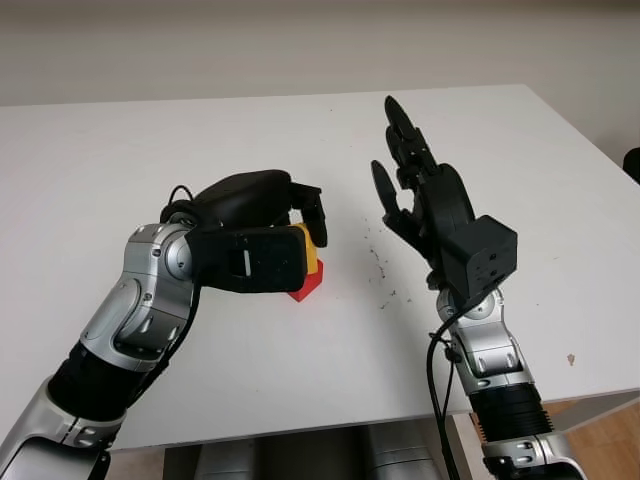
\includegraphics[width=\linewidth]{figures/cosmos/ep000_f450_original.png}
    \caption{Original}
  \end{subfigure}\hspace{0.04\linewidth}
  \begin{subfigure}[t]{0.37\linewidth}
    \centering
    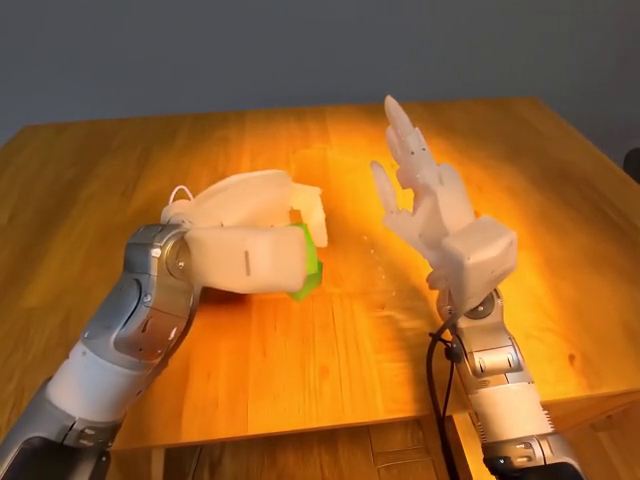
\includegraphics[width=\linewidth]{figures/cosmos/ep000_f450_variante0.png}
    \caption{Stilvariante \enquote{warmes Licht, Holztisch}}
  \end{subfigure}
  \caption[Stilvariante von Cosmos-Transfer2.5]{Linke Kopfkamera, Episode~0, Frame~450:
    Original und stärkste Stilvariante.}
  \label{fig:cosmos-varianten}
\end{figure}

Haltung und Bildaufbau bleiben erhalten; die Variante in \cref{fig:cosmos-varianten} färbt aber
auch die schwarzen Hände weiß und einen Würfel grün, obwohl der Prompt den Roboter unverändert lassen soll.
